% CSE 455/555 final report (main file by Vaishak, R6; restructured to the course's 3-4 page
% format with introduction and references by Sanika, R5).
% Build from report/:  latexmk -pdf main.tex   (or pdflatex, bibtex, pdflatex, pdflatex)
% Every number comes from results/; see README.md to regenerate it.
\documentclass[conference]{IEEEtran}
\usepackage[utf8]{inputenc}
\usepackage[T1]{fontenc}
\usepackage{graphicx}
\usepackage{booktabs}
\usepackage{amsmath}
\usepackage{cite}                       % numbered IEEE citations, sorted and compressed: [2]-[4]
\usepackage[hidelinks]{hyperref}

\begin{document}

\title{Bandwidth-Limited Pattern Recognition: Which Induction-Motor Fault Signatures
Survive Consumer-Grade Vibration Sensing?}

\author{\IEEEauthorblockN{Vaishak G Kumar and Sanika Vilas Najan}
\IEEEauthorblockA{Department of Engineering Science (Artificial Intelligence), University at
Buffalo, Buffalo, NY, USA\\ vaishakg@buffalo.edu, snajan@buffalo.edu}}

\maketitle

\begin{abstract}
A smartphone on a motor samples vibration at 100\,Hz, so the textbook signatures of a cracked
bearing race and of voltage imbalance, both above 50\,Hz, are lost or aliased. We ask which of
six induction-motor health states remain separable, using 126 hand-written features,
hand-implemented PCA, LDA and Kernel PCA, and six classical classifiers on 36 public recordings,
with whole recordings held out over five seeds. A random split over windows scores up to 1.00
macro-F1; on unseen recordings the best model reaches $0.47 \pm 0.03$ (chance 0.17). LDA's
Fisher ratio falls from about 490 in-sample to 15 held-out, because it mostly learns which
recording a window came from. Lubrication loss survives through impulsiveness, while rotor-bar
sidebands coincide with aliased shaft harmonics at 50\,Hz supply. Models trained on clean data
collapse under 10\% noise or dropout, and an unseen load breaks the PCA front-ends unless each
condition is normalised separately.
\end{abstract}

% R5: introduction and dataset (Sanika). Builds on the proposal's problem statement.

\section{Introduction and Dataset}\label{sec:intro}

Electric motor systems used 53\% of the world's electricity in 2023, 72\% in industry
\cite{iea2025}. Vibration monitoring catches bearing and rotor faults before they cause a
failure, but the standard diagnostics demodulate bearing-defect frequencies from accelerometers
sampled at kilohertz rates \cite{randall2011}. The common benchmark, the Case Western Reserve
bearing data, is sampled at 12 and 48\,kHz, and standard envelope analysis already diagnoses
many of its faults \cite{smith2015}. Small workshops and farms skip that equipment and run motors to
failure. A smartphone is already at every machine, but its inertial sensor logs at about 100\,Hz.

At 100\,Hz nothing above the 50\,Hz Nyquist frequency survives \cite{shannon1949}: it is removed
or folded back into the band. For the motor studied here (shaft speed $f_1 \approx 15$, 20 and 25\,Hz), the
outer-race defect frequency of a cracked bearing (44--86\,Hz) and the twice-line-frequency
signature of voltage imbalance (60--100\,Hz) lie above that limit, while the rotor-bar sidebands
at $f_1 \pm 2sf_\mathrm{supply}$ \cite{nandi2005} and the impulsiveness caused by poor lubrication
lie below it.
The usual question, which classifier is best, therefore turns into a different one (Track 2:
dimensionality reduction against noise and out-of-distribution data): \emph{which class
structure survives the truncation, which projection preserves it, and how does it hold up when
the sensor degrades or the operating condition changes?} Answering it needs an honest test.
Overlapping windows cut from one recording are near-copies, and random splits over windows
overstate vibration-diagnosis accuracy \cite{wheat2024}, a case of the leakage that inflates
machine-learning results across fields \cite{kapoor2023}, so every result here holds out whole
recordings and is repeated over five seeds. We contribute (i) a separability boundary: which
fault information a 100\,Hz sensor keeps, which it hides, and why; (ii) the size of the leakage
gap, from 1.00 macro-F1 on random splits to 0.47 on unseen recordings; and (iii) how the
projections hold up under sensor corruption, an unseen speed or load, and domain adaptation.
Sections~\ref{sec:methods}--\ref{sec:conclusion} give the methods, results and conclusions.

\textbf{Related work.} Classical pipelines pair hand-crafted time- and frequency-domain features
with PCA or LDA and a shallow classifier \cite{duda2001}; Kernel PCA \cite{scholkopf1998} is the
non-linear variant, Subspace Alignment \cite{fernando2013} adapts such a subspace to a new
operating condition, and DTW \cite{sakoe1978} compares waveforms without features. We test each
at 100\,Hz on held-out recordings.

\textbf{Dataset.} We use the public (CC BY 4.0) dataset of Ertar{\u{g}}{\i}n et al.~\cite{ertargin2026}. An iPhone 15 Pro Max lies on
a squirrel-cage induction motor and logs six inertial channels at 100\,Hz: the raw accelerations
$g_X, g_Y, g_Z$ and the gravity-compensated user accelerations $g^u_X, g^u_Y, g^u_Z$. There are
six health states: healthy (H), insufficient lubrication (B1), severely insufficient lubrication
(B2), a cracked outer bearing ring (B3), supply-voltage imbalance (V) and a broken rotor bar (R).
Each class is recorded once at each of six operating conditions (supply frequency 30, 40 or
50\,Hz, unloaded or loaded), giving 36 balanced recordings of about 15 minutes (90{,}000 samples
per channel).

\textbf{Pre-processing.} Each recording is cut into windows of 1{,}024 samples (10.24\,s, a
0.098\,Hz frequency resolution) with a 512-sample step: 6{,}264 labelled windows, 174 per
recording. The mean of each window is removed per channel, which drops gravity and sensor
offset. Amplitudes are not normalised, because absolute vibration energy is discriminative;
every scaling step is fitted inside the cross-validation folds.

% Methodology (R1 by Vaishak, condensed to the 4-page format in R5). Pipeline in src/motorpr/
% (features.py, projections.py, kernel_pca.py, evaluation.py, corruption.py, domain.py,
% analysis.py, dtw.py, tuning.py).

\section{Methodology}\label{sec:methods}

\textbf{Features.} Each window yields 21 hand-written features per channel, 126 in all. Eight
are time-domain statistics: RMS, variance, skewness, kurtosis, crest factor, peak-to-peak, shape
factor and impulse factor. Thirteen are spectral and are measured relative to the shaft speed
$f_1$, estimated per window as the strongest periodogram peak between 0.80 and 1.03 times the
synchronous speed (it drops 4--8\% under load): the energy fractions at $f_1$ and $2f_1$, a sideband fraction
0.5--3\,Hz either side of $f_1$, four band powers (below $0.5f_1$, around $f_1$, around $2f_1$,
above $2.5f_1$), the Welch \cite{welch1967} spectral centroid, spread and entropy, the maximum and
mean spectral kurtosis \cite{antoni2006}, and the slip $1 - f_1/f_\mathrm{sync}$. There is no separate feature-selection step:
the projections below reduce the dimension, and Sec.~\ref{sec:separability} analyses which
features carry the separability.

\textbf{Projections.} After standardisation, each pipeline applies one of five front-ends, all
implemented by hand \cite{duda2001}: none (126-D), PCA keeping 95\% of the variance, PCA to five dimensions,
Fisher LDA \cite{fisher1936} to five dimensions ($C-1$ for six classes), and RBF Kernel PCA to five dimensions.
LDA solves $S_B v = \lambda S_W v$ with $S_W$ shrunk by the Ledoit--Wolf estimate
\cite{ledoit2004}, since features that are nearly constant within a recording make it singular.
Kernel PCA \cite{scholkopf1998} centres the kernel $\exp(-\gamma\lVert x-x'\rVert^2)$ with
$\gamma = 1/126$, keeps its top five eigenvectors, and is fitted on at most 1{,}500 training
windows.

\textbf{Classifiers and hyperparameters.} Each front-end feeds six scikit-learn \cite{pedregosa2011}
classifiers: $k$-NN with $k=5$ (Euclidean, and Mahalanobis via Ledoit--Wolf whitening) and
Gaussian naive Bayes \cite{duda2001}, a linear SVM ($C=1$) and an RBF SVM ($C=10$,
$\gamma = 1/(d\,\mathrm{Var}(x))$) \cite{cortes1995}, and a random forest of 300 trees
\cite{breiman2001}: 30 pipelines, each fitted on the training fold only. To check that these defaults do not
limit accuracy, every classifier on the raw, LDA-5 and Kernel PCA-5 front-ends is also tuned by
nested grouped cross-validation \cite{cawley2010}: five inner grouped folds inside each outer
training fold search the neighbour count, $C$, the RBF width, the forest leaf size, the naive
Bayes smoothing and the Kernel PCA $\gamma \in \{0.002, 1/126, 0.03\}$.

\textbf{Validation.} We compare three splits. \emph{Naive}: stratified folds over windows; it
leaks near-duplicate windows and only measures that leakage. \emph{Grouped} (main protocol):
each class's six recordings are dealt one per fold, so every test fold holds one whole unseen
recording per class. \emph{Leave one condition out}: fold $k$ holds out every class at operating
condition $k$. Scores are macro-F1 over six folds (chance $1/6$). Fold-to-fold spread reaches
$\pm0.2$, so every experiment is repeated over five seeds (fold assignment, forest seed, Kernel
PCA subsample, corruption noise) and reported as mean $\pm$ std. Separability is scored on
held-out recordings with a transfer Fisher ratio $J$ \cite{fisher1936, duda2001}: the between-class scatter comes from the
training class means, the within-class scatter from held-out windows around those means.

\textbf{Robustness.} Three sensor failures are applied to each whole raw recording before
windowing, at levels 0--0.5: additive white noise with variance equal to the level times the
channel's vibration variance (0.5 is an SNR of 3\,dB); sample dropout in contiguous 5--50-sample
gaps filled by linear interpolation, as in Bluetooth packet loss; and a per-axis gain that
drifts linearly over the recording. Models are either trained and tested on corrupted data, or
trained clean and tested corrupted. Two fixed splits
isolate unseen conditions: train on 30 and 50\,Hz and test on 40\,Hz, and train unloaded and test
loaded. There we compare Subspace Alignment \cite{fernando2013}, which aligns the source PCA
basis to the target's using unlabelled target windows, with per-domain z-scoring alone and with
no adaptation.

\textbf{Analysis and DTW.} The separability analysis scores each feature for each of the 15
class pairs with the transfer $J$, measures the rotor-bar sidebands at $f_1 \pm f_p$
($f_p = 2sf_\mathrm{supply}$) on 0.012\,Hz whole-recording spectra, and splits window energy into
regions relative to $f_1$, including aliased shaft and line harmonics. Dynamic time warping
\cite{sakoe1978} is tested as a $k$-NN distance between window envelopes (log RMS of 16-sample
frames, band $\pm 8$). These analyses and the tuning use seed~0.

% Results and discussion (R5: condensed from R1 by Vaishak and R2-R4 by Sanika).
% 5-seed numbers: scripts/aggregate_seeds.py + make_methods_tables.py (tab_grid,
% fig_corruption) and make_report_figures.py (fig_projection, fig_kpca left); seed-0 numbers:
% run_analysis.py, run_dtw.py, run_tuning.py.

\section{Results and Discussion}\label{sec:results}

\subsection{Leakage, model comparison and the projections}

\begin{table*}[t]
  \centering
  \caption{Grouped cross-validation: macro-F1 of every front-end and classifier (mean
  $\pm$ std over 5 seeds; chance 0.17). Bold: best.}
  \label{tab:grid}
  \begin{tabular}{lcccccc}
\toprule
Front-end & $k$-NN & $k$-NN (Mah.) & Lin.\ SVM & RBF SVM & RF & GNB \\
\midrule
Raw 126-D & 0.28 $\pm$ 0.03 & 0.25 $\pm$ 0.04 & \textbf{0.47 $\pm$ 0.03} & 0.35 $\pm$ 0.04 & 0.39 $\pm$ 0.05 & 0.27 $\pm$ 0.02 \\
PCA (95\% var.) & 0.29 $\pm$ 0.01 & 0.30 $\pm$ 0.03 & 0.41 $\pm$ 0.02 & 0.38 $\pm$ 0.03 & 0.40 $\pm$ 0.03 & 0.27 $\pm$ 0.06 \\
PCA-5 & 0.28 $\pm$ 0.03 & 0.23 $\pm$ 0.01 & 0.31 $\pm$ 0.04 & 0.36 $\pm$ 0.04 & 0.29 $\pm$ 0.04 & 0.24 $\pm$ 0.03 \\
LDA-5 & 0.45 $\pm$ 0.06 & 0.42 $\pm$ 0.06 & 0.44 $\pm$ 0.07 & 0.43 $\pm$ 0.05 & 0.42 $\pm$ 0.05 & 0.43 $\pm$ 0.06 \\
Kernel PCA-5 & 0.15 $\pm$ 0.01 & 0.16 $\pm$ 0.02 & 0.28 $\pm$ 0.05 & 0.20 $\pm$ 0.02 & 0.21 $\pm$ 0.06 & 0.21 $\pm$ 0.03 \\
\bottomrule
\end{tabular}

\end{table*}

\begin{figure*}[t]
  \centering
  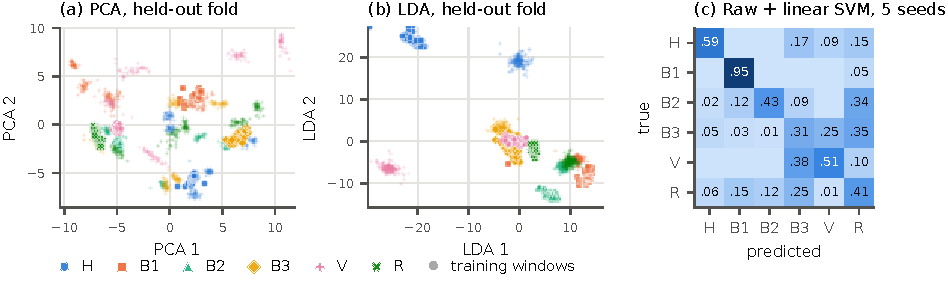
\includegraphics[width=\textwidth]{figures/fig_projection.pdf}
  \caption{(a, b) PCA and LDA fitted on one grouped fold's training recordings (small dots); large
  markers: the six held-out recordings, which land beside LDA's tight training clusters, not in
  them. (c) Row-normalised confusion matrix of the best model, pooled over 5 seeds.}
  \label{fig:projection}
\end{figure*}

\begin{figure*}[t]
  \centering
  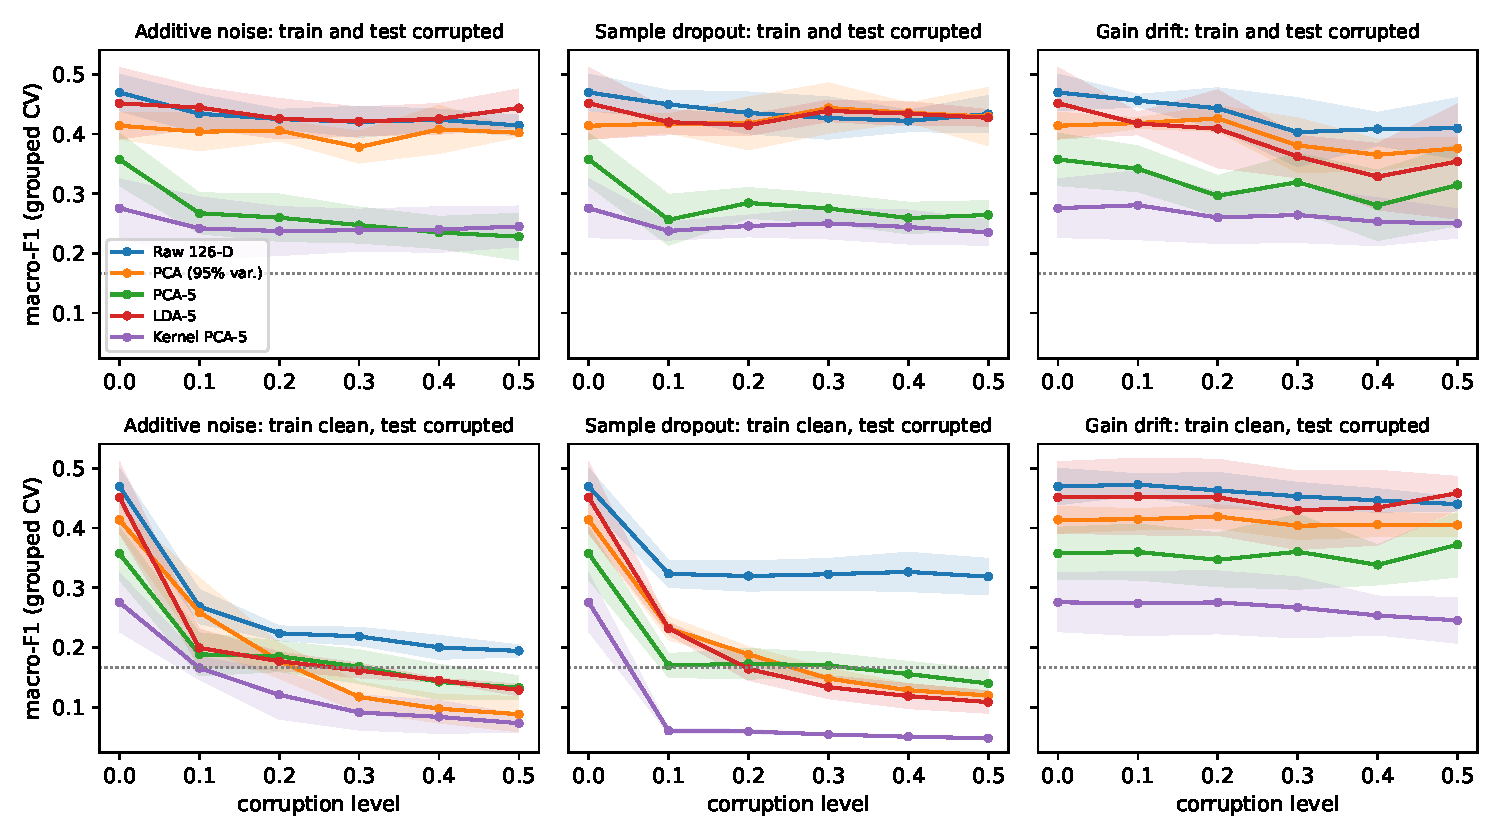
\includegraphics[width=0.6\textwidth]{figures/fig_corruption.pdf}
  \caption{Best macro-F1 per front-end against corruption level (grouped CV, 5 seeds, $\pm$1 std).
  Top: training and test corrupted alike; bottom: clean training, corrupted test; dotted: chance.}
  \label{fig:corruption}
\end{figure*}

Holding out whole recordings matters most: under the naive split 26 of the 30 models
score 0.99 or higher; with whole recordings held out none exceeds 0.47
(Table~\ref{tab:grid}), and leaving one condition out gives at most 0.56. The best model is the
linear SVM on the raw features ($0.47 \pm 0.03$). A max-margin linear boundary can combine many
weak cues across all 126 features, while the distance-based $k$-NN does poorly on the raw space
(0.25--0.28), where every feature counts equally, and well after LDA (0.42--0.45), which
reweights features by class separation. LDA-5 is decent with every classifier but not ahead over five
seeds (its seed-0 best, 0.49 with a random forest, does not hold). Separability on the training data misleads: LDA's Fisher $J$ at $k=5$ is about 490 in-sample but $15.1 \pm 4.7$ on held-out recordings, against $10.1 \pm 3.5$ for PCA. Most of what it
separates on its training fold is which recording a window came from (Fig.~\ref{fig:projection}b).
Per class (Fig.~\ref{fig:projection}c), B1 is recognised almost perfectly (recall 0.95), while H,
B3 and V blur together, and B2 is often taken for R (0.34).

\subsection{What survives a 100\,Hz sensor}\label{sec:separability}

Scored per class pair along the two-class LDA direction, the held-out $J$ is 0.4--7.4 against
600--1{,}600 in-sample. \textbf{B1 separates from every class} ($J$ 2.2--7.4), and against H
through impulsiveness: kurtosis ($J = 7.5$), peak-to-peak (4.7) and impulse factor (4.1). Poor
lubrication makes the vibration impulsive, and time-domain statistics capture that without any
defect frequency. No single feature separates any class from all five others (best weakest-pair $J$: 0.76).

\textbf{R is not separated by its rotor-bar sidebands,} the textbook broken-bar signature
\cite{nandi2005}. The sideband feature integrates
0.5--3\,Hz either side of $f_1$, but the measured pole-pass spacing is 3.5--10.1\,Hz under load
and below 0.5\,Hz unloaded, so it misses the real sidebands in all 36 recordings. Measured
directly, R's sidebands are never the strongest at their condition (rank 3, 6 and 4 of 6 under
load). At 50\,Hz supply they also coincide exactly with aliased shaft harmonics, for any slip:
for a four-pole motor $f_1 + f_p = 100 - 3f_1$, the alias of $3f_1$, and $f_1 - f_p$ is the alias
of $5f_1$. A 100\,Hz sensor cannot tell them apart. R's one consistent cue is slip under load
(median 0.056 against 0.043--0.047 for H and the bearing classes), hence the R$\leftrightarrow$B2
confusion.

\textbf{B3 and V} are defined by frequencies above Nyquist. Twice the line frequency folds to DC
at 50\,Hz supply and onto $f_1$ at 40\,Hz. H and V are best told apart by the energy at
\emph{aliased shaft-harmonic} positions ($J = 2.75$), mechanical harmonics folded down from above
50\,Hz, and V slips most under load (median 0.101). No spectral region separates B3 from H
($J \le 0.21$); its best single feature is skewness ($J = 1.11$), a waveform asymmetry rather
than a spectral line. These numbers are seed 0.

\subsection{Sensor corruption and unseen conditions}

The two deployments behave in opposite ways (Fig.~\ref{fig:corruption}). Corrupted alike,
noise and dropout barely matter even at 50\%. Gain drift hurts, and it hurts LDA most ($0.45 \to 0.35$ at level 0.5), because
the per-recording gain breaks the absolute amplitude cues LDA relies on. Trained clean, the
picture reverses: 10\% noise or dropout drops every projected front-end to 0.17--0.26 and Kernel
PCA to 0.06--0.17, while gain drift barely matters, since most features are scale-free ratios.
The raw features degrade least (0.32 at every dropout level). Corruption shifts the feature distribution (kurtosis, spectral kurtosis, entropy) rather than
erasing the classes, and projections fitted on clean data are the most
brittle to that shift, Kernel PCA most of all.

A new speed is easy: trained on 30 and 50\,Hz, the best model reaches $0.66 \pm 0.02$ at 40\,Hz.
A new load is the hard shift, because loading lowers the shaft speed and moves the whole harmonic
comb. Both PCA front-ends fall to 0.14--0.15 and Kernel PCA to 0.05; the raw features and LDA-5
keep about 0.40. B1 survives the load change (recall 0.92) while R falls to 0.16: its
load-dependent slip was never seen in training. Adaptation lifts the unseen load from 0.14--0.18
to 0.42--0.60, mostly through z-scoring each domain with its own statistics; Subspace Alignment
adds little and in either direction ($-0.07$ to $+0.09$ against z-scoring). The shift is mostly
a change of location and scale per feature.

\subsection{Kernel PCA, tuning and DTW}

\begin{figure}[t]
  \centering
  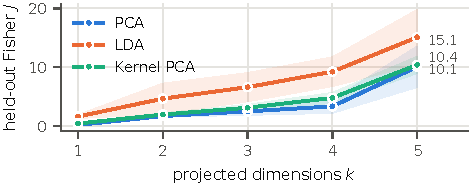
\includegraphics[width=\columnwidth]{figures/fig_fisher_k.pdf}
  \caption{Held-out Fisher $J$ against $k$ (5 seeds, mean $\pm$ std).}
  \label{fig:kpca}
\end{figure}

The non-linear projection does not help. Kernel PCA keeps as much held-out separability as PCA
at every $k$ ($10.4 \pm 1.5$ against $10.1 \pm 3.5$ at $k=5$; Fig.~\ref{fig:kpca}), yet its best
classifier reaches only $0.28 \pm 0.05$. With $\gamma = 1/126$, two standardised windows sit
about 16 apart, where the kernel is already down to 0.13, so the embedding emphasises local
neighbourhoods of the training recordings. Consistent with that, nested tuning most often picks
the wider $\gamma = 0.002$, which brings Kernel PCA closer to linear PCA. Tuning in general changes
little (seed 0, every second training window): on the raw and LDA-5 front-ends the gain over
the defaults lies between $-0.03$ and $+0.04$, inside the fold-to-fold spread of 0.10--0.17, and
for most models the selected setting changes from fold to fold. The largest gain, Kernel PCA-5
with an RBF SVM (0.22 to 0.35),
still leaves it below the linear front-ends. Elastic alignment brings nothing either: DTW on the
window envelopes scores $0.28 \pm 0.07$ against $0.26 \pm 0.09$ without warping and
$0.30 \pm 0.12$ for the features (seed 0): windows of a steady run start at arbitrary shaft
phases, so there is nothing to align. The envelope beats the features on R (recall 0.61 against 0.23)
but not on B1 (0.54 against 0.97).

% R6: conclusion (Vaishak). Summarises Sections III-VIII; no new numbers.

\section{Conclusion}\label{sec:conclusion}

We asked which induction-motor fault signatures survive a 100\,Hz smartphone sensor, and
measured it on recordings the models had never seen. The answer is a boundary rather than an
accuracy:
\begin{itemize}
  \item \textbf{Survives.} Lubrication loss (B1) separates from every other class through
        impulsiveness (kurtosis, peak-to-peak, impulse factor), with no defect frequency needed,
        and it survives a change of load.
  \item \textbf{Hidden by the sensor.} The rotor-bar sidebands of R fall outside the band our
        sideband feature integrates and, at 50\,Hz supply, coincide exactly with aliased
        running-speed harmonics for any slip. R's one consistent cue is its slip under load,
        which a model trained only on unloaded data cannot use.
  \item \textbf{Above Nyquist.} The defining frequencies of B3 and V lie above 50\,Hz; what
        separates them weakly is waveform asymmetry, slip and aliased mechanical harmonics, not
        their own signatures.
\end{itemize}

Several negative results are findings in their own right. A random split over windows reports
near-perfect accuracy that disappears when whole recordings are held out. LDA's large in-sample
separability is mostly recording identity. A single seed made LDA with a random forest look
best; averaged over five seeds, a linear SVM on the raw features is. Kernel PCA, elastic
alignment (DTW) and nested hyperparameter tuning do not move the result, and most of the gain
from Subspace Alignment comes from normalising each operating condition separately.

\textbf{Limitations.} Each class is recorded once per operating condition on one motor and one
phone, so recording-to-recording variation within a class is barely sampled: this, rather than
model capacity, limits accuracy. The bearing defect frequencies assume a 6204-type bearing
because the dataset does not name it. Subspace Alignment and per-domain z-scoring use unlabelled
windows from the new condition.

\textbf{Future work.} Several recordings per class and condition, more than one motor and phone,
and a sensor sampling above 200\,Hz would show whether the boundary is a property of the faults
or of this setup.

\textbf{Reproducibility.} The full pipeline re-runs from the raw data with the commands in the
repository README: download the 36 recordings, extract features, run every experiment over five
seeds, aggregate, and regenerate every table and figure in this report. Each results folder
records its seed, parameters, library versions and the dataset version.


\bibliographystyle{IEEEtran}
\bibliography{references}

\end{document}
